\documentclass[12pt]{beamer}
%\usepackage{fontspec}
\usepackage[spanish]{babel}
\usepackage[utf8]{inputenc}
%\usepackage{authblk}
%Código
\usepackage{listings}
\usepackage{xcolor}
\usepackage{caption}
\captionsetup[lstlisting]{labelformat=empty}% redefines the caption setup of the figures environment in the beamer class.
\captionsetup[figure]{labelformat=empty}
\usepackage{spverbatim}
\usepackage{fancyvrb}
\usepackage{fvextra}
%Imágenes
\usepackage{graphicx}
\graphicspath{{img/}}
\usepackage{float}
\usepackage{adjustbox}



% the various libraries we will be using
\usepackage{tikz}
\usetikzlibrary{calc}
\usepackage[none]{hyphenat}
\usepackage{longtable}
\usepackage{booktabs}

\usepackage{array}
\newcolumntype{L}[1]{>{\raggedright\let\newline\\\arraybackslash\hspace{0pt}}m{#1}}
\newcolumntype{C}[1]{>{\centering\let\newline\\\arraybackslash\hspace{0pt}}m{#1}}
\newcolumntype{R}[1]{>{\raggedleft\let\newline\\\arraybackslash\hspace{0pt}}m{#1}}

% macro
\def\BeginColumn#1{\begin{columns}\column{#1\textwidth}}
\def\Column#1{\column{#1\textwidth}}
\def\EndColumn{\end{columns}}
\providecommand{\tightlist}{%
    \setlength{\itemsep}{0pt}\setlength{\parskip}{0pt}}

% define colours
% taken from pickton on Adobe Kuler:
% https://kuler.adobe.com/Some-Kind-Of-Execushares-color-theme-3837185/
\definecolor{ExecusharesBlue}{RGB}{153,204,255}
\definecolor{ExecusharesBlack}{RGB}{43,40,40}
\definecolor{ExecusharesWhite}{RGB}{255,255,243}
\definecolor{ExecusharesGrey}{RGB}{107,110,108}

% set colours
\setbeamercolor{itemize item}{fg=ExecusharesBlue}
\setbeamercolor{enumerate item}{fg=ExecusharesBlue}
\setbeamercolor{alerted text}{fg=ExecusharesBlue}
\setbeamercolor{section in toc}{fg=ExecusharesBlack}

% set fonts
\setbeamerfont{itemize/enumerate body}{size=\large}
\setbeamerfont{itemize/enumerate subbody}{size=\normalsize}
\setbeamerfont{itemize/enumerate subsubbody}{size=\small}

% make the itemize bullets pixelated >
\setbeamertemplate{itemize item}{
  \tikz{
    \draw[fill=ExecusharesBlue,draw=none] (0, 0) rectangle(0.1, 0.1);
    \draw[fill=ExecusharesBlue,draw=none] (0.1, 0.1) rectangle(0.2, 0.2);
    \draw[fill=ExecusharesBlue,draw=none] (0, 0.2) rectangle(0.1, 0.3);
  }
}
% make the subitems also pixelated >, but a little smaller and Blue
\setbeamertemplate{itemize subitem}{
  \tikz{
    \draw[fill=ExecusharesBlue,draw=none] (0, 0) rectangle(0.075, 0.075);
    \draw[fill=ExecusharesBlue,draw=none] (0.075, 0.075) rectangle(0.15, 0.15);
    \draw[fill=ExecusharesBlue,draw=none] (0, 0.15) rectangle(0.075, 0.225);
  }
}

% disable navigation
\setbeamertemplate{navigation symbols}{}

% custom draw the title page above
\setbeamertemplate{title page}{}

% again, manually draw the frame title above
\setbeamertemplate{frametitle}{}

% disable "Figure:" in the captions
\setbeamertemplate{caption}{\tiny\insertcaption}
%\setbeamertemplate{caption label separator}{ }

% since I don't know a better way to do this, these are all switches
% doing `\setcounter{showProgressBar}{0}` will turn the progress bar off (I turn it off for Appendix slides)
% etc
\newcounter{showProgressBar}
\setcounter{showProgressBar}{1}
\newcounter{showSlideNumbers}
\setcounter{showSlideNumbers}{1}
\newcounter{showSlideTotal}
\setcounter{showSlideTotal}{1}

% use \makeatletter for our progress bar definitions
% progress bar idea from http://tex.stackexchange.com/a/59749/44221
% slightly adapted for visual purposes here
\makeatletter
\newcount\progressbar@tmpcounta% auxiliary counter
\newcount\progressbar@tmpcountb% auxiliary counter
\newdimen\progressbar@pbwidth %progressbar width
\newdimen\progressbar@tmpdim % auxiliary dimension

\newdimen\slidewidth % auxiliary dimension
\newdimen\slideheight % auxiliary dimension

% make the progress bar go across the screen
%\progressbar@pbwidth=12.8cm
\progressbar@pbwidth=\the\paperwidth
\slidewidth=\the\paperwidth
\slideheight=\the\paperheight

% use tikz to draw everything
% it may not be the best, but it's easy to work with
% and looks good
% TODO: base title slide and contents slide on something other than slide numbers :/
\setbeamertemplate{background}{
  % deal with progress bar stuff
  % (calculate where it should go)
  \progressbar@tmpcounta=\insertframenumber
  \progressbar@tmpcountb=\inserttotalframenumber
  % \advance\progressbar@tmpcounta by -1
  % \advance\progressbar@tmpcountb by -1
  \progressbar@tmpdim=\progressbar@pbwidth
  \multiply\progressbar@tmpdim by \progressbar@tmpcounta
  \divide\progressbar@tmpdim by \progressbar@tmpcountb

  \begin{tikzpicture}
    % set up the entire slide as the canvas
    \useasboundingbox (0,0) rectangle(\the\paperwidth,\the\paperheight);

    % the background
    \fill[color=ExecusharesWhite] (0,0) rectangle(\the\paperwidth,\the\paperheight);

    % separate the drawing based on if we're the first (title) slide or not
    \ifnum\thepage=1\relax
      % the title page
      % draw the fills
      \fill[color=ExecusharesBlue] (0, 4cm) rectangle(\slidewidth,\slideheight);

      % draw the actual text
      \node[anchor=south,text width=\slidewidth-1cm,inner xsep=0.5cm] at (0.5\slidewidth,4cm) {\color{ExecusharesWhite}\Huge\textbf{\inserttitle}};
      \node[anchor=north east,text width=\slidewidth-1cm,align=right] at (\slidewidth-0.4cm,4cm) {\color{ExecusharesBlack}\tiny\insertsubtitle};
      \node[above] at(0.5\slidewidth,2.3cm) {\color{ExecusharesBlack}\tiny };
      \node at (0.5\slidewidth,2cm) {\color{ExecusharesBlack}\Large\insertauthor};

      % add the date in the corner
      \node[anchor=south east] at(\slidewidth,0cm) {\color{ExecusharesGrey}\tiny\insertdate};
    \else
      % NOT the title page
      % title bar
      \fill[color=ExecusharesBlue] (0, \slideheight-1cm) rectangle(\slidewidth,\slideheight);

      % swap the comment on these to add section titles to slide titles
      %\node[anchor=north,text width=11.8cm,inner xsep=0.5cm,inner ysep=0.25cm] at (6.4cm,9.6cm) {\color{ExecusharesWhite}\Large\textbf{\insertsectionhead: \insertframetitle}};
      \node[anchor=north,text width=\slidewidth-1cm,inner xsep=0.5cm,inner ysep=0.25cm] at (0.5\slidewidth,\slideheight) {\color{ExecusharesWhite}\huge\textbf{\insertframetitle}};
      
      % if we're showing a progress bar, show it
      % (I disable the progress bar and slide numbers for the "Appendix" slides)
      \ifnum \value{showProgressBar}>0\relax%
        % the the progress bar icon in the middle of the screen
        \draw[fill=ExecusharesGrey,draw=none] (0cm,0cm) rectangle(\slidewidth,0.25cm);
        \draw[fill=ExecusharesBlue,draw=none] (0cm,0cm) rectangle(\progressbar@tmpdim,0.25cm);

        % bottom information
        \node[anchor=south west] at(0cm,0.25cm) {\color{ExecusharesGrey}\tiny\insertsection};
        % if slide numbers are active
        \ifnum \value{showSlideNumbers}>0\relax%
          % if slide totals are active
          \ifnum \value{showSlideTotal}>0\relax%
            % draw both slide number and slide total
            \node[anchor=south east] at(\slidewidth,0.25cm) {\color{ExecusharesGrey}\tiny\insertframenumber/\inserttotalframenumber};
          \else
            % slide totals aren't active, don't draw them
            \node[anchor=south east] at(\slidewidth,0.25cm) {\color{ExecusharesGrey}\tiny\insertframenumber};
          \fi
        \fi
      % don't show the progress bar?
      \else
        % section title in the bottom left
        \node[anchor=south west] at(0cm,0cm) {\color{ExecusharesGrey}\tiny\insertsection};
        % if we're showing slide numbers
        \ifnum \value{showSlideNumbers}>0\relax%
          % if slide totals are active
          \ifnum \value{showSlideTotal}>0\relax%
            % draw both slide number and slide total
            \node[anchor=south east] at(\slidewidth,0cm) {\color{ExecusharesGrey}\tiny\insertframenumber/\inserttotalframenumber};
          \else
            % slide totals aren't active, don't draw them
            \node[anchor=south east] at(\slidewidth,0cm) {\color{ExecusharesGrey}\tiny\insertframenumber};
          \fi
        \fi
      \fi
    \fi
  \end{tikzpicture}
}
\makeatother

% add section titles
\AtBeginSection{\frame{\sectionpage}}
\setbeamertemplate{section page}
{
  \begin{tikzpicture}
    % set up the entire slide as the canvas
    \useasboundingbox (0,0) rectangle(\slidewidth,\slideheight);
    %\fill[color=ExecusharesWhite] (0,0) rectangle(\the\paperwidth,\the\paperheight);
    \fill[color=ExecusharesWhite] (-1cm, 2cm) rectangle (\slidewidth, \slideheight+0.1cm);
    \fill[color=ExecusharesBlue] (-1cm, 0.5\slideheight-1cm) rectangle(\slidewidth, 0.5\slideheight+1cm);
    \node[text width=\the\paperwidth-1cm,align=center] at (0.4\slidewidth, 0.5\slideheight) {\color{ExecusharesWhite}\Huge\textbf{\insertsection}};
  \end{tikzpicture}
}

% source code syntax highlight
\usepackage{color}
\usepackage{fancyvrb}
\newcommand{\VerbBar}{|}
\newcommand{\VERB}{\Verb[commandchars=\\\{\}]}
\DefineVerbatimEnvironment{Highlighting}{Verbatim}{commandchars=\\\{\}}
% Add ',fontsize=\small' for more characters per line
\newenvironment{Shaded}{}{}
\newcommand{\KeywordTok}[1]{\textcolor[rgb]{0.00,0.44,0.13}{\textbf{{#1}}}}
\newcommand{\DataTypeTok}[1]{\textcolor[rgb]{0.56,0.13,0.00}{{#1}}}
\newcommand{\DecValTok}[1]{\textcolor[rgb]{0.25,0.63,0.44}{{#1}}}
\newcommand{\BaseNTok}[1]{\textcolor[rgb]{0.25,0.63,0.44}{{#1}}}
\newcommand{\FloatTok}[1]{\textcolor[rgb]{0.25,0.63,0.44}{{#1}}}
\newcommand{\ConstantTok}[1]{\textcolor[rgb]{0.53,0.00,0.00}{{#1}}}
\newcommand{\CharTok}[1]{\textcolor[rgb]{0.25,0.44,0.63}{{#1}}}
\newcommand{\SpecialCharTok}[1]{\textcolor[rgb]{0.25,0.44,0.63}{{#1}}}
\newcommand{\StringTok}[1]{\textcolor[rgb]{0.25,0.44,0.63}{{#1}}}
\newcommand{\VerbatimStringTok}[1]{\textcolor[rgb]{0.25,0.44,0.63}{{#1}}}
\newcommand{\SpecialStringTok}[1]{\textcolor[rgb]{0.73,0.40,0.53}{{#1}}}
\newcommand{\ImportTok}[1]{{#1}}
\newcommand{\CommentTok}[1]{\textcolor[rgb]{0.38,0.63,0.69}{\textit{{#1}}}}
\newcommand{\DocumentationTok}[1]{\textcolor[rgb]{0.73,0.13,0.13}{\textit{{#1}}}}
\newcommand{\AnnotationTok}[1]{\textcolor[rgb]{0.38,0.63,0.69}{\textbf{\textit{{#1}}}}}
\newcommand{\CommentVarTok}[1]{\textcolor[rgb]{0.38,0.63,0.69}{\textbf{\textit{{#1}}}}}
\newcommand{\OtherTok}[1]{\textcolor[rgb]{0.00,0.44,0.13}{{#1}}}
\newcommand{\FunctionTok}[1]{\textcolor[rgb]{0.02,0.16,0.49}{{#1}}}
\newcommand{\VariableTok}[1]{\textcolor[rgb]{0.10,0.09,0.49}{{#1}}}
\newcommand{\ControlFlowTok}[1]{\textcolor[rgb]{0.00,0.44,0.13}{\textbf{{#1}}}}
\newcommand{\OperatorTok}[1]{\textcolor[rgb]{0.40,0.40,0.40}{{#1}}}
\newcommand{\BuiltInTok}[1]{{#1}}
\newcommand{\ExtensionTok}[1]{{#1}}
\newcommand{\PreprocessorTok}[1]{\textcolor[rgb]{0.74,0.48,0.00}{{#1}}}
\newcommand{\AttributeTok}[1]{\textcolor[rgb]{0.49,0.56,0.16}{{#1}}}
\newcommand{\RegionMarkerTok}[1]{{#1}}
\newcommand{\InformationTok}[1]{\textcolor[rgb]{0.38,0.63,0.69}{\textbf{\textit{{#1}}}}}
\newcommand{\WarningTok}[1]{\textcolor[rgb]{0.38,0.63,0.69}{\textbf{\textit{{#1}}}}}
\newcommand{\AlertTok}[1]{\textcolor[rgb]{1.00,0.00,0.00}{\textbf{{#1}}}}
\newcommand{\ErrorTok}[1]{\textcolor[rgb]{1.00,0.00,0.00}{\textbf{{#1}}}}
\newcommand{\NormalTok}[1]{{#1}}

\title{Criptografía de la curva elíptica}
\author[Author One at al.]{\makebox[0pt]{Sofía Almeida \and Pedro Flores \and Victoria Granados}} 
%\date{\today}


\setbeamertemplate{frametitle continuation}{\gdef\beamer@frametitle{}}

\begin{document}
\frame{\titlepage}

\frame{\tableofcontents}

\section{Curva elíptica}\label{curva}
\large
\begin{frame}[fragile]{Curva elíptica}
  Consideramos un cuerpo $K$ y definimos la curva elíptica $E$ sobre él de la siguiente forma:
\normalsize
\[E = \{(x,y) \in K\times K : y^2 = x^3 + ax +b,\ 4a^3+27b \neq 0\} \cup \{\infty\}.
\]
\large
El punto $\infty$ se añade por definición.
\end{frame}

\begin{frame}[fragile]{Curva elíptica}
\begin{lstlisting}[ label={cod:ej1}, caption={Curva elíptica $y^2=x^3-x$},language=Python, morekeywords={sage}]
sage: E =  EllipticCurve(RR, [-1, 0]);
      plot(E, (-4, 3), color=hue(0.6))
\end{lstlisting}

\begin{figure}[H]
    \centering
    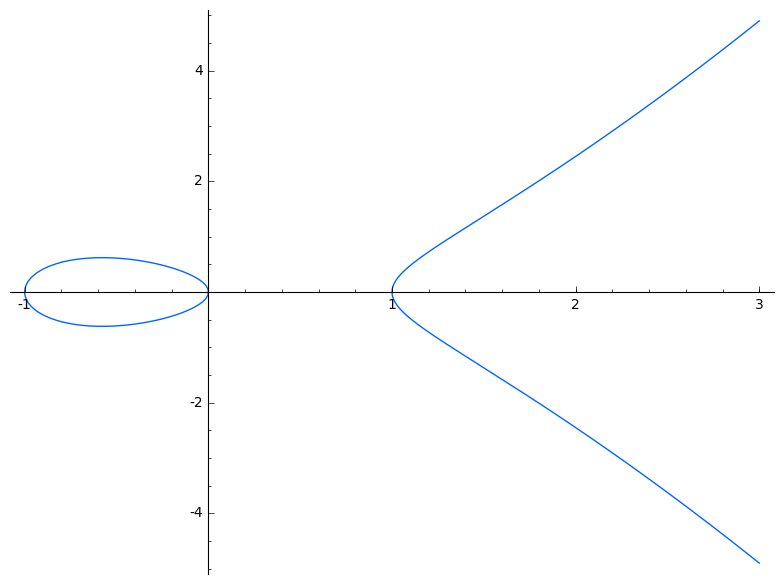
\includegraphics[height=0.4\textwidth, width=0.4\textwidth]{ej1}
    \label{fig:ej1}
\end{figure}

\end{frame}

\begin{frame}[fragile]{Curva elíptica}
\begin{figure}[H]
    \centering
    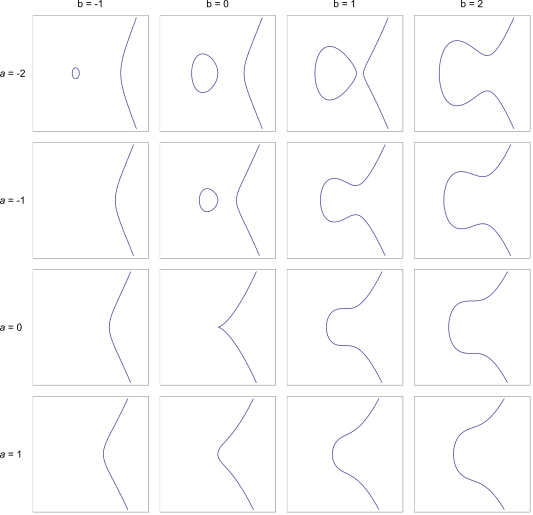
\includegraphics[width=0.62\textwidth]{EllipticCurveCatalog}
    \label{fig:EllipticCurveCatalog}
\end{figure}
\end{frame}

\begin{frame}[fragile]{Estructura de grupo}
  \begin{itemize}
  \item Elemento neutro: $\infty$.
  \item Elemento opuesto de $ P = (x_P, y_P) $: $-P = (x_P, -y_P) $.
  \item Operación de suma: P + Q = R.
  \end{itemize}
\end{frame}

\begin{frame}[fragile]{Estructura de grupo}
  \begin{itemize}
  \item Operación de suma: P + Q = R.
  \end{itemize}
    \begin{figure}[H]
	\centering
	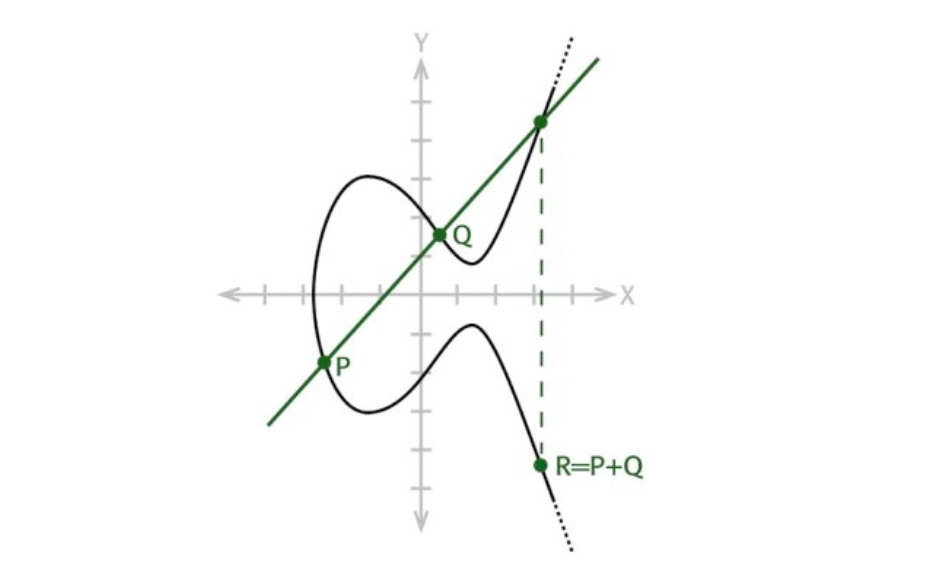
\includegraphics[width=0.8\textwidth]{ec_add}
	\label{fig:EC_add}
\end{figure}
\end{frame}

\begin{frame}[fragile]{Estructura de grupo}
  \begin{itemize}
  \item Elemento neutro: $\infty$.
  \item Elemento opuesto de $ P = (x_P, y_P) $: $-P = (x_P, -y_P) $.
  \item Operación de suma: P + Q = R.
  \item Producto por escalares, $n \in \mathbb{Z}$: \[   
nP = 
\begin{cases}
 (P+\stackrel{n}{\cdots}+P) &\text{si } n > 0\\
0 &\text{si } n = 0\\
(-P-\stackrel{n}{\cdots}-P) &\text{si } n < 0\\
\end{cases}.
\]
  \end{itemize}
\end{frame}

\begin{frame}[fragile]{EC sobre cuerpos finitos}
  \begin{align*}
    E = \{(x,y) \in  \mathbb{F}_p \times \mathbb{F}_p :& y^2 \equiv x^3 + ax +b \bmod p,\\
    & 4a^3+27b \not\equiv 0 \bmod p\} \cup \{\infty\}.
\end{align*}
  
  \begin{figure}[H]
	\centering
	\begin{minipage}[b]{0.45\textwidth}
	\centering
	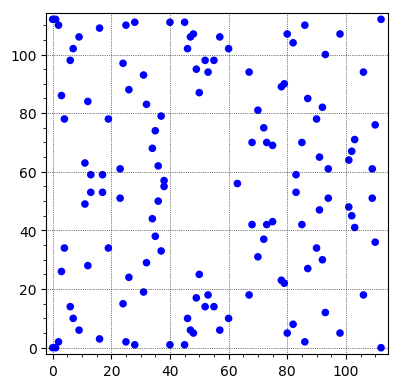
\includegraphics[width=0.7\textwidth]{EC_F_113}
	\caption{$y^2 + y=x^3-x $ sobre $ \mathbb{F}_{113}$}
	\label{fig:ej5}
	\end{minipage}
	\begin{minipage}[b]{0.45\textwidth}
		\centering
	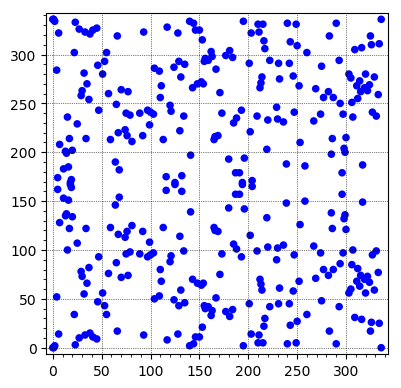
\includegraphics[width=0.7\textwidth]{EC_F_337}
	\caption{$y^2 + y=x^3-x $ sobre $ \mathbb{F}_{337} $}
	\label{fig:ej6}
	\end{minipage}
\end{figure}
\end{frame}

\begin{frame}[fragile]{Subgrupos}
  \begin{itemize}
  \item Los múltiplos de $P$ generan un subgrupo cíclico de orden $\min\{ n \in \mathbb{N}:\text{ } nP = \infty \text{ y } n | N\}$.\\
    
  \item Primero elegimos el orden del subgrupo, $n$, y posteriormente hallamos el generador $P$.
  \end{itemize}
  
\end{frame}

\section{Problema del logaritmo discreto}\label{dis_log}
\begin{frame}[fragile]{Problema del logaritmo discreto}
Si conocemos $ P $ y $ Q $ dos puntos de la curva elíptica, ¿podemos encontrar un $ k $ tal que $ Q = kP $?  
\end{frame}
\begin{frame}[fragile]{Problema del logaritmo discreto}
Si conocemos $ P $ y $ Q $ dos puntos de la curva elíptica, ¿podemos encontrar un $ k $ tal que $ Q = kP $?\\
\vspace{3mm}
  
No existe demostración que pruebe su dificultad.\\
\vspace{3mm}

Algoritmo \textit{Baby-step, giant-step}, complejidad $O(\sqrt{n})$.\\
\end{frame}

\section*{Algoritmos}
\begin{frame}[fragile]{Parámetros}
  \begin{itemize}
	\item $ p $: número primo.
	\item $ a, b $: coeficientes de la curva elíptica.
	\item $ G $: generador del subgrupo.
	\item $ n $: orden del subgrupo.
	\item $ h $:  cofactor del subgrupo, $h = N / n$.
\end{itemize}
\end{frame}

\begin{frame}[fragile]{Claves}
 \begin{itemize}
\item Clave privada: entero aleatorio $d$ elegido en el intervalo $[1,n-1]$.
\item Clave pública: punto de la curva $H = dG$.
\end{itemize}
\end{frame}

\section{ECDH}\label{ecdh}

\begin{frame}[fragile]{ECDH}
 \vspace{5mm}
  \begin{enumerate}
  \item Generación de claves:\\
   \quad Claves de Alice: $d_A$ y $H_A = d_AG$.\\
   \quad Claves de Bob: $d_B$ y $H_B = d_BG$. 

\item Alice y Bob intercambian sus claves públicas.\\
\item Cálculo de clave compartida:\\
  \quad Alice calcula $C = d_AH_B$.\\
  \quad Bob calcula $C = d_BH_A$.\\
  \[C = d_AH_B = d_A(d_BG) = d_B(d_AG) = d_BH_A = C.\]
\end{enumerate}

\end{frame}

\section{ECDSA}\label{ecdsa}
\begin{frame}[fragile]{ECDSA - Firma}
\vspace{5mm}
  \begin{enumerate}
	\item  Elegimos $ k $ entero aleatorio en el conjunto $ \{ 1, ..., n-1\} $.
	\item Calculamos \textit{P} = \textit{kG}.
	\item Hallamos el número \textit{$r \equiv x_{P} \mod n$}.
	\item Si \textit{r} es 0 volvemos al paso 1.
	\item Calculamos $s \equiv k^{-1}(z + rd_{A}) \mod n$.
	\item Si \textit{s} es 0 volvemos a 1.
  \end{enumerate}
  \vspace{2mm}
  La firma será: (\textit{r}, \textit{s}).
  
\end{frame}

\begin{frame}[fragile]{ECDSA - Verificación}
\begin{enumerate}
	\item Calculamos $u_1 \equiv$ \textit{$s^{-1}$ z} mod\textit{n}.
	\item Calculamos $u_2 \equiv$ \textit{$s^{-1}$ r} mod\textit{n}.
	\item Calculamos el punto $P = u_1G + u_2 H_A$.	
\end{enumerate}

\vspace{2mm}
  La firma es válida si $r \equiv x_P \mod n$.

\end{frame}

\begin{frame}[fragile]{ECDSA - Importancia de $k$}
  \begin{enumerate}
	\item $r_1$ es igual a $r_2$, puesto que $ r \equiv x_P \mod n$ y $P = kG$ es el mismo para las dos firmas.
	\item  $(s_1 - s_2) \mod n \equiv k^{-1} (z_1 - z_2) \mod n$.
	\item $k  \equiv (z_1 - z_2) (s_1 -s_2)^{-1} \mod n$.
        \item Despejamos $d_S$ de $s \equiv k^{-1}(z + r d_S) \mod n$ y obtenemos $d_S \equiv r^{-1}(sk - z) \mod n$, todos valores conocidos. 
\end{enumerate}
\end{frame}

\section{Curvas elípticas más utilizadas}\label{ej_curvas}

\begin{frame}[fragile, allowframebreaks=0.8]{Curvas elípticas más utilizadas}
  \begin{itemize}
\item Spec256k1 (o Curve25519): se utiliza para ECDSA en el modelo criptográfico de Bitcoin. Viene dada por:
\[
y^2 = x^3 + 7.
\]
Se suele utilizar como punto base
\begin{align*}
G = (0\texttt{x}&\text{79be667ef9dcbbac55a06295ce870b07} \\
				&\text{029bfcdb2dce28d959f2815b16f81798}, \\
	 0\texttt{x}&\text{483ada7726a3c4655da4fbfc0e1108a8} \\
	 			&\text{fd17b448a68554199c47d08ffb10d4b8}),
\end{align*}
que nos aporta un grupo de orden
\[
2^{256}-0\texttt{x}\text{14551231950b75fc4402da1732fc9bebf}.
\]

\item NIST P-256: es la que trae \textit{OpenSSL} por defecto y existen una gran cantidad de métodos para optimizar su uso. \\

\item Curve25519: es una de las curvas más rápidas que existen actualmente y su implementación de referencia es de dominio público. Viene dada por
\[
y^2 = x^3 + 48662x^2 + x
\]
definida sobre el cuerpo finito con $ 2^{255} - 19 $ elementos y el punto base tal que $ x = 9 $. Esto nos aporta un subgrupo de orden 
\[  2^{252 }+ 0\texttt{x}\text{14def9dea2f79cd65812631a5cf5d3ed}. \]

\item  Curve448: ofrece potencialmente 224 bits de seguridad y aporta un gran rendimiento. Su implementación base está disponible bajo una licencia MIT. \\
\end{itemize}

\end{frame}

\section{Comparación con RSA}\label{rsa}
\normalsize
\begin{frame}[fragile]{Comparación con RSA}
  \begin{table}[H]
	  \centering
	  \begin{adjustbox}{width=\textwidth}
	    \begin{tabular}{L{3cm}rR{3cm}}
	  \toprule
	   & \textbf{RSA} & \textbf{EC} \\
	  \midrule
	  \textbf{Problema en que basa su seguridad} & Factorización & Logaritmo discreto\\
	  \textbf{Almacenamiento de claves} & 1024 & 160\\
           & 153600 & 521 \\
	  \bottomrule
	\end{tabular}
	\end{adjustbox}
	\end{table}
\end{frame}

\section{Demostración práctica}\label{demo}
\normalsize
\begin{frame}[fragile]{OpenSSL}
\begin{Verbatim}[breaklines=true]
  $ openssl ecparam -list_curves
  $ openssl ecparam -name secp256k1 -out secp256k1.pem
  $ cat secp2561.pem
  $ openssl ecparam -in secp256k1.pem -genkey -noout -out secp256k1-key.pem
  $ cat secp256k1-key.pem 
  $ openssl ecparam -name secp256k1 -genkey -noout -out secp256k1-key.pem
  $ cat secp256k1-key.pem
  $ openssl ec -in secp256k1-key.pem -pubout -out ecpubkey.pem
\end{Verbatim}

\end{frame}
\end{document}
